\documentclass[conference]{IEEEtran}
\IEEEoverridecommandlockouts
% The preceding line is only needed to identify funding in the first footnote. If that is unneeded, please comment it out.
\usepackage{cite}
\usepackage{amsmath,amssymb,amsfonts}
% \usepackage{algorithmic}
\usepackage{graphicx}
\usepackage{textcomp}
\usepackage{xcolor}
\usepackage{multirow}

\graphicspath{{./Figures/}}
\def\BibTeX{{\rm B\kern-.05em{\sc i\kern-.025em b}\kern-.08em
    T\kern-.1667em\lower.7ex\hbox{E}\kern-.125emX}}
\begin{document}

\title{Chest Abnormalities Detection and Localization - Final Report \\
}

\author{\IEEEauthorblockN{Kanstantsin Pachkouski}
\IEEEauthorblockA{\textit{Electrical and Computer Engineering} \\
\textit{Western University}\\
London, Canada \\
kpachkou@uwo.ca}
\and
\IEEEauthorblockN{Kyle Rioux}
\IEEEauthorblockA{\textit{Electrical and Computer Engineering} \\
\textit{Western university}\\
London, Canada \\
krioux5@uwo.ca}
\and
\IEEEauthorblockN{Christopher Tam}
\IEEEauthorblockA{\textit{Electrical and Computer Engineering} \\
\textit{Western University}\\
London, Canada \\
ctam86@uwo.ca}
}

\maketitle

\begin{abstract}
    Current automated approaches for examining chest X-rays lack accuracy and list only entire-image findings without descriptive localization. An automated method to accurately identify chest X-ray abnormalities with localization in the image would therefore be an invaluable tool in providing improved healthcare globally. Thus, we developed a computer-aided tool that is able to perform accurate detection of 14 common chest X-ray abnormalities with bounding boxes. In addition, each detected abnormality will have a confidence percentage associated with it. In this report, we evaluate three R-CNN models and a YOLO model for object detection and localization with heavy preprocessing steps taken. Upon competition completion, our team scored a mean absolute precision (mAP) of 24.6\% placing us in the top 26\% of all teams. 
\end{abstract}

\section{Introduction} \label{intro}
Diagnostic medical imaging is an invaluable tool in the treatment of patients around the world. The development of imaging modalities such as CT, MRI, PET, and X-ray have allowed healthcare professionals to gain critical information which would be otherwise unavailable or require an invasive procedure. Although some images are relatively easy to interpret and can be done by a general practitioner, in many cases, it takes a radiologist to draw diagnosis from the complex images.
It is well known that there is a global radiologist shortage, especially in developing countries \cite{rimmer2017radiologist}. The development of computer programs to analyze complex medical images could greatly reduce the burden on healthcare systems all around the world and lead to improved patient outcomes.

Among the most complex and common medical images is the chest X-ray. As X-rays are far cheaper than alternative imaging modalities such as CT, MRI, or PET, they are much more commonly used in developing countries. As the chest X-ray includes a large portion of the body, there are many conditions which are identified utilizing the chest X-ray. Current automated chest X-ray interpretation techniques are able to identify what they believe is present in an image, but give no localization as to where they believe the finding is within the image; this leads to a low level of interoperability and could add to the confusion of a doctor reviewing findings of the automated system. 

We aim to develop a computer-aided diagnostics system which is able to perform detection on 14 common findings within a chest x-ray by localizing them in the image with a region of interest (ROI) bounding box, as well as a confidence percentage. For example, the system may provide the output similar to the following:  ‘The system is 70\% sure that there is a nodule in this location’. This additional information will provide increased interpretability to computer-aided diagnostics systems and will allow them to fit more readily into current clinical workflows. 

The content of this report is organized as follows: Section \ref{related_work} presents a description of the object detection and localization methods used in this project along with a review of the previous contributions made to those models. Section \ref{dataset} presents an overview of the dataset used for this project, describing the data gathering and annotation process. Section \ref{methodology} presents our exploratory data analysis results, data preprocessing steps, model construction, hyperparameter tuning process, and training and validation efforts. Section \ref{results_and_analysis} presents how we quantified our results from Section \ref{methodology} and provides a benchmark comparison of our group to other groups in the competition, and Section \ref{future_work} summarizes our project findings and presents ideas for future work.

\section{Related Work} \label{related_work}
Previous work in object detection tasks with localization have used R-CNN, or Regions with CNN Features networks. R-CNN is an object detection model that applies high-capacity CNNs to bottom-up region proposals in order to localize and segment objects \cite{girshick2014rich}. R-CNN uses selective search to identify a number of bounding-box object region candidates, and extracts features from each region independently for classification. R-CNN can be broken down into three modules. The first module generates category-independent region proposals which define the set of candidate regions available to the detector. The second module is a CNN responsible for extracting a fixed-length feature vector from each of the candidate regions. The third module consists of a set of class-specific linear SVMs. This novel approach of combining region proposals with CNNs heavily outperformed previous best performing models which relied on combining multiple low-level image features with high-level context. R-CNN gave a 30\% relative improvement over the best previous results on the Pascal Visual Object Classes Challenge 2012 (PASCAL VOC 20212) competition. 

Although R-CNN made a significant contribution to object detection with localization, it had several notable drawbacks. First, training R-CNN involved a multi-stage process. R-CNN first fine-tuned a ConvNet on object proposals and then fit SVMs to the ConvNet features. Bounding-box regressors were not learned until after fitting SVMs in the third training stage. Second, training R-CNN is expensive in space and time. For SVM and bounding-box regressor training, every feature extracted from each region proposal was written to disk. According to the authors, this process took 2.5 GPU-days of training for the 5k images of the VOC07 trivial set using the VGG-16 deep network. These features required hundreds of gigabytes of storage. Third, object detection is slow. VGG-16 took an average of 47 seconds per image to make predictions on the test set. 

In 2015, Girshick proposed Fast R-CNN \cite{girshick2015fast}, an improvement over R-CNN by aggregating regions of interest into a single forward pass over the image. In this context, regions of interest from the same image share computation in the forward and backward passes. Specifically, Fast R-CNN improves R-CNN in the following ways. First, the detection quality is improved. Second, training is done in a single stage (as opposed to the multi-stage process described above). Third, during training Fast R-CNN is able to update all network layers. Finally, no disk storage is required for feature caching thereby greatly improving memory requirements. In order to train Fast R-CNN, the network takes images and a set of object proposals as input. Several convolutional and max pooling layers are used to produce a convolutional feature map for each of the object proposals. An RoI pooling layer then extracts a fixed-length feature vector from the feature map for each of the object proposals, which are then fed into a sequence of fully connected layers that branch into two output layers. The first branch produces a softmax probability over all the target object classes, and the second branch outputs a set of four real-valued numbers for each of the target object classes. These four real-value numbers represent the bounding-box positions describing the region where a target object class was found. Fast R-CNN was again evaluated on the VOC 2012 dataset, the same dataset its predecessor made a breakthrough on. Fast R-CNN achieved a mean average precision (or, mAP, will be discussed extensively in Results and Analysis) of 65.7\%, improving over its predecessor by 6\%. Fast R-CNN was also two orders of magnitude faster than other methods based on the comparably slower R-CNN pipeline.

Later, Faster R-CNN \cite{ren2015faster} was proposed as an improvement over Fast R-CNN. Faster R-CNN introduces a Region Proposal Network (RPN) that shares full-image convolutional features with the detection network. RPN is a fully convolutional network that simultaneously predicts object bounds with their associated probabilities at each position, thus enabling nearly cost-free region proposals. RPN is used in conjunction with Fast R-CNN through shared convolutional features. As such, Faster R-CNN can be seen as consisting of two distinct modules. The RPN network tells the unified network where to look and the Fast R-CNN detector uses the proposed regions to make predictions. Faster R-CNN achieved a mAP of 67\%, improving over its predecessor by 2\% after being trained on the public VGG-16 model.

Faster R-CNN models have been successfully combined with multiple CNN architectures; one of which is the MobileNet \cite{howard2017mobilenets}. As the name suggests, MobileNet was originally created with mobile and embedded applications in mind. MobileNet has the goal of generating more lightweight and efficient neural networks to account for the limited processing power available for inference on mobile devices. This is achieved by building models which are appropriately sized depending on the constraints of the problem.  MobileNet has been known to find comparable results to alternative CNN’s with much faster training and inference times due to the simplified architecture.

The You Only Look Once (YOLO) \cite{redmon2016you} model is an alternative object recognition framework which has seen extensive success. YOLO models are based on the idea that entire images are seen at once during both training and testing, hence “only looking once”. This is done by framing the object detection as a regression problem which has inputs as images, and outputs of recognized object’s bounding boxes and associated confidence probabilities. As a result of this architectural change, there is no need for separate region proposal and object detection networks as is present in some of the previous models. This network is exceptionally fast, operating at real time speeds of 45-150fps and achieves double the mAP of other real time detectors. YOLO models make more localization errors than some state of the art algorithms, but are less prone to false positives in the background; as reducing false positives is extremely important in our abnormality detection problem, we believe this will be an ideal model candidate.

\section{Dataset} \label{dataset}
This project uses the VinDr-CXR open dataset \cite{nguyen2020vindr} of chest X-rays with radiologist annotations, collected by researchers at the Vingroup Big Data Institute from the Hospital 108 (H108) and the Hanoi Medical University Hospital (HMUH), two of the largest hospitals in Vietnam. This dataset consists of 18,000 postero-anterior view chest X-ray scans that come with both the localization of critical findings and the classification of 14 common thoracic diseases. These images were annotated by a group of 17 radiologists with at least 8 years of experience for the presence of the diseases found in the dataset. The Vingroup researchers divided the dataset into two parts: the training set of 15,000 scans and the test set of 3,000 scans. Each image in the training set was independently labeled by 3 radiologists, while the annotation of images in the test set were obtained through the consensus findings of 5 radiologists. 

The Vingroup researchers provided labels for the training set in the form Comma-Separated Values (CSV) file format. Each entry in this file provides information about the ID of the radiologist who made a prediction, name of the image, class ID and coordinates specifying the position of the bounding box. Since each X-ray in the training set was annotated independently, consensus was not reached among radiologists and disagreements occurred. For example, an image could have been labeled by three radiologists and each of them might have found a different set of abnormalities in the image. Images in the test set were labeled by five radiologists in a two-stage process. Each image was first annotated by three doctors independently, followed by two other doctors with higher levels of expertise. Doctors reviewed the findings and communicated with each other to reach a consensus about the labels in the image. Therefore, it should be noted that images in the training set might have incorrect labels, and that images in training and testing sets were labeled using different approaches.

\section{Methodology} \label{methodology}
\subsection{Exploratory Analysis}
We first analyzed the Class and Radiologist IDs data. The distribution of abnormalities and radiologists, who labeled the images, is presented in Figure \ref{fig:numImages}. As seen from the figure, certain radiologists contributed far more than the others. In addition, the training set has unequal class distribution. 
\begin{figure}[h]
	\centering
    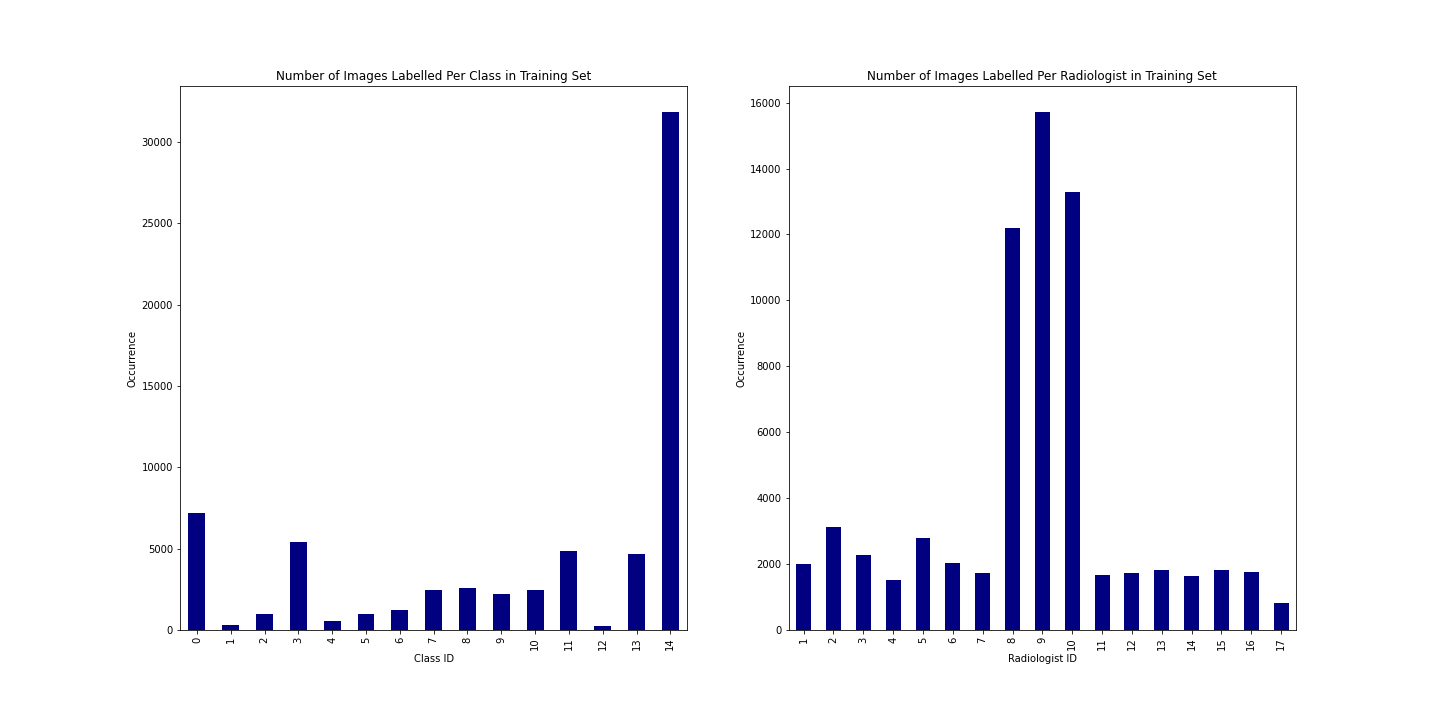
\includegraphics[width=0.80\linewidth]{NumImagesPerClassAndRad}
    \caption{Number of images per class and number of images per radiologist}
	\label{fig:numImages}
\end{figure}

\begin{figure}[h]
	\centering
    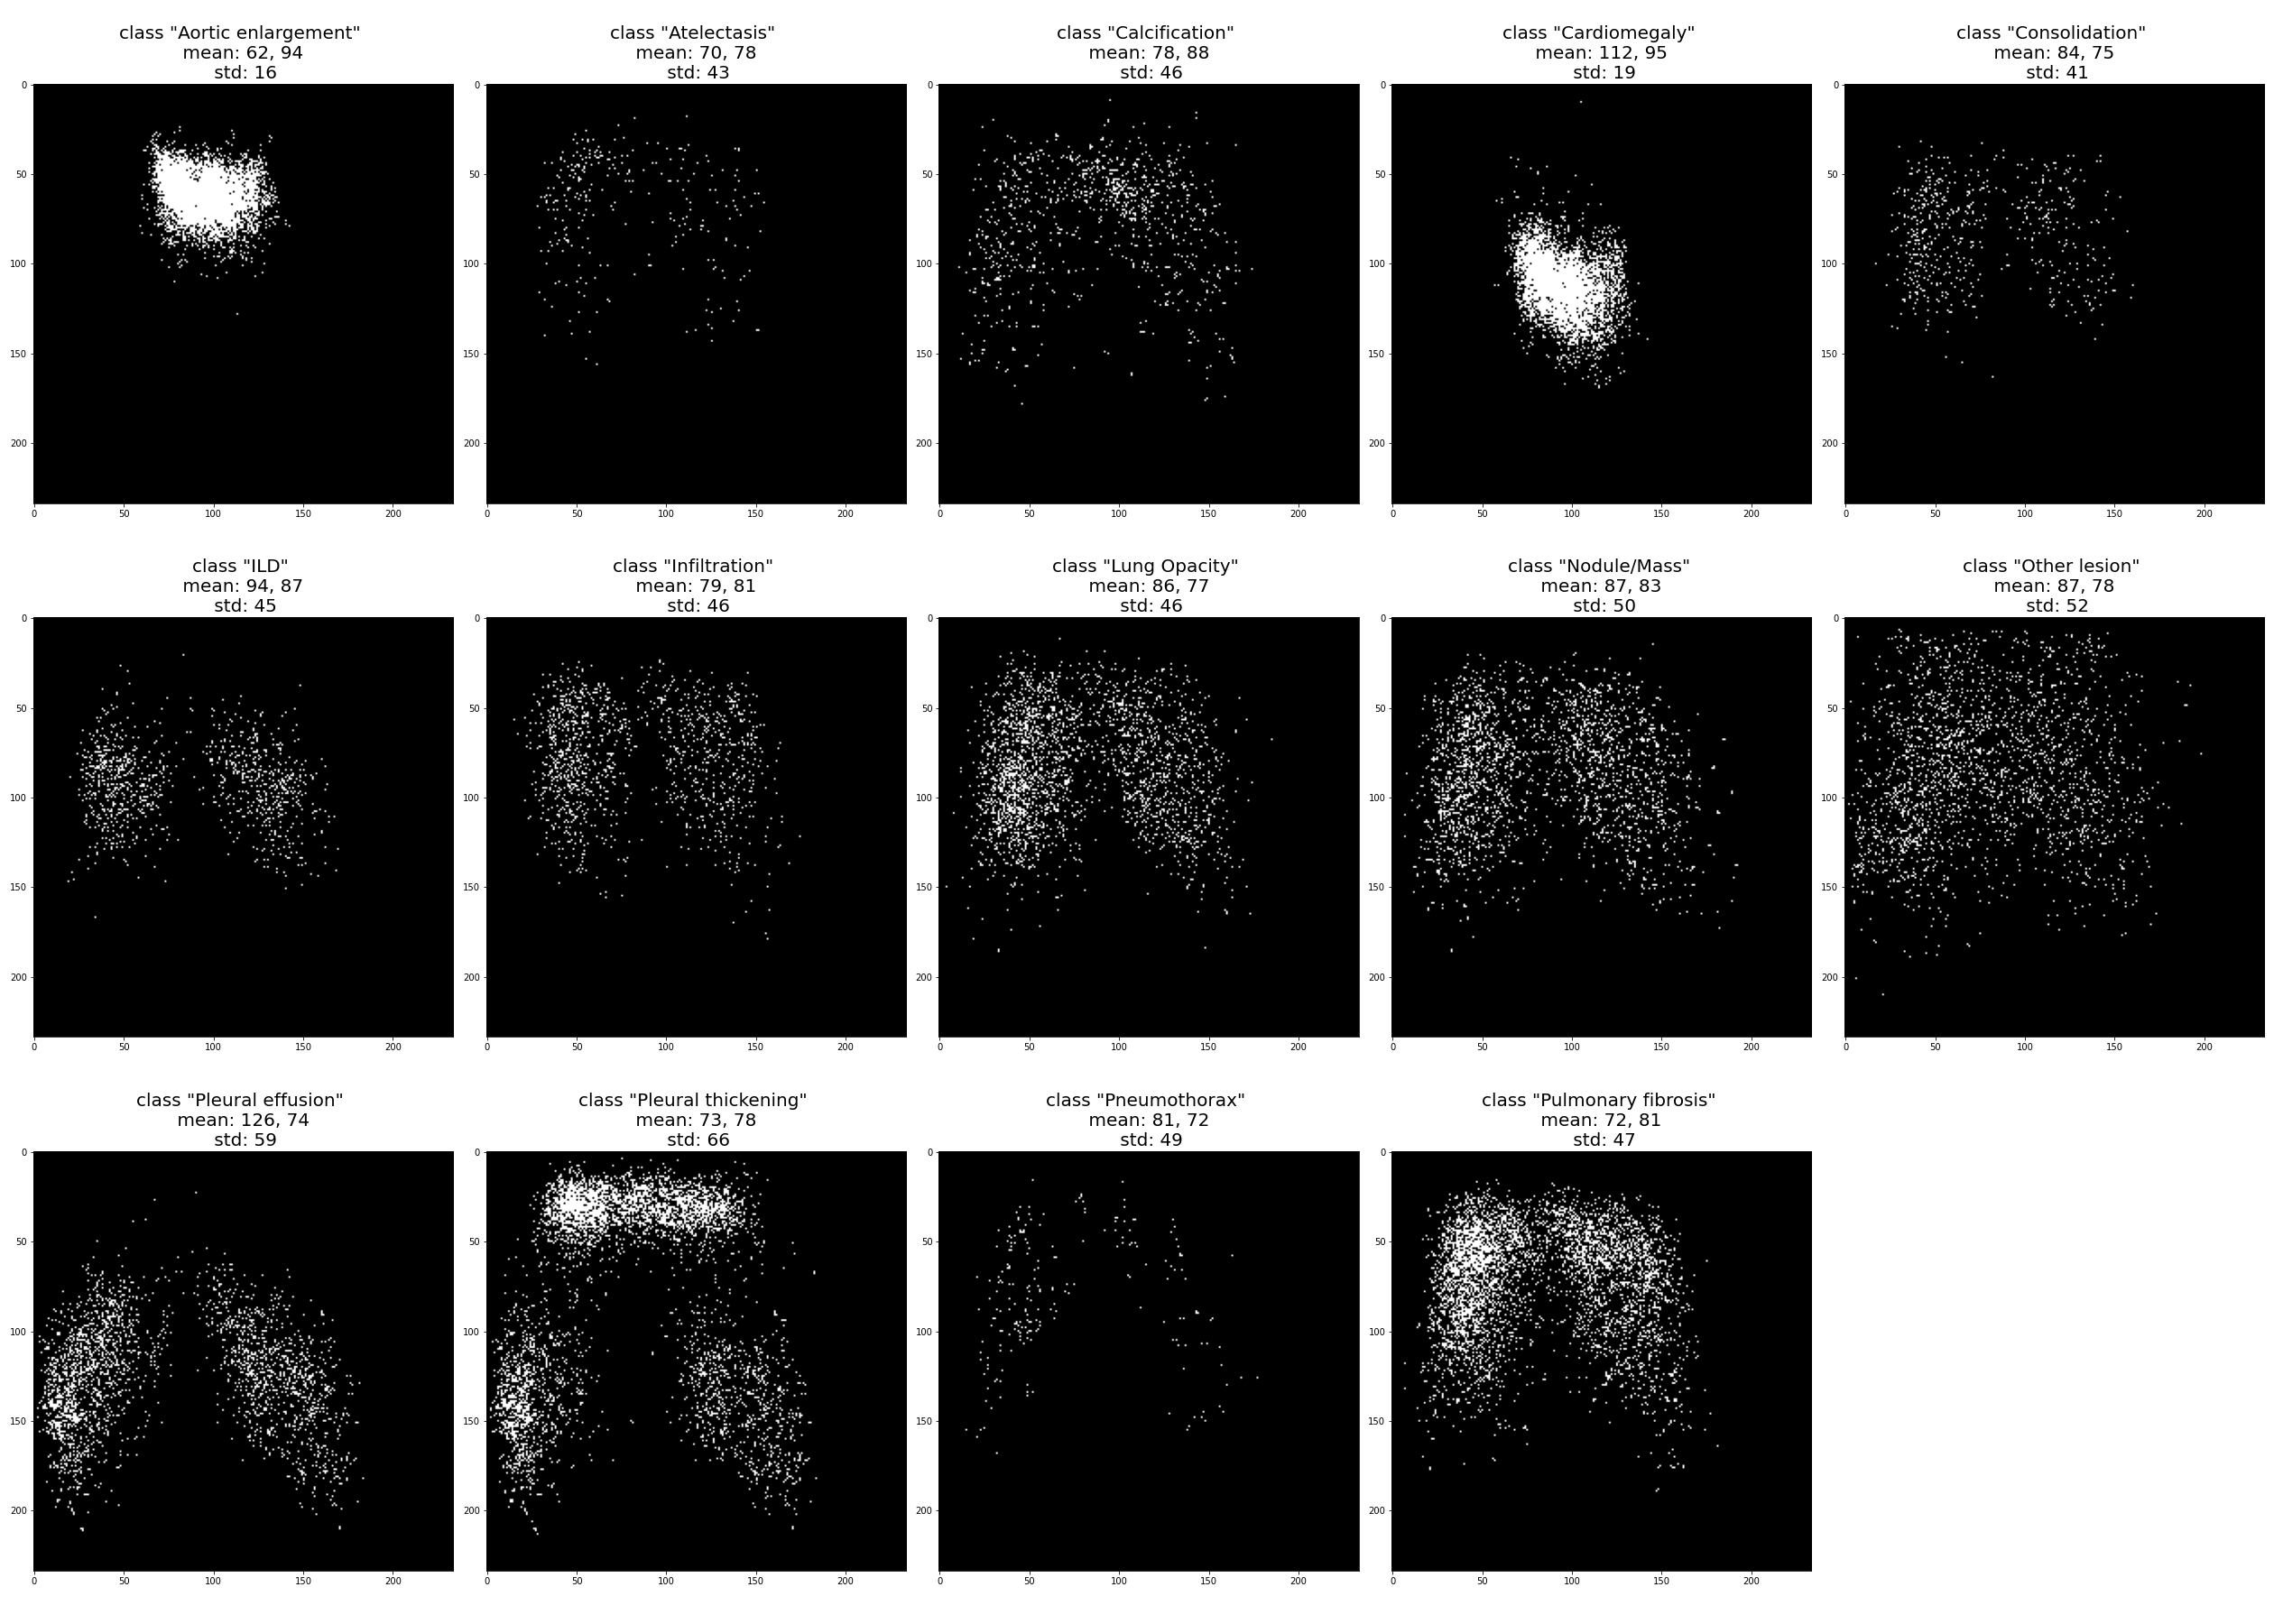
\includegraphics[width=0.80\linewidth]{bounding_box_distr-5}
    \caption{Distribution of bounding box locations}
	\label{fig:distBB}
\end{figure}

\begin{figure}[h]
	\centering
    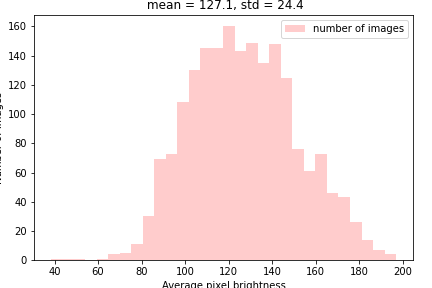
\includegraphics[width=0.80\linewidth]{DistAvgBrightness}
    \caption{Distribution of average image brightness}
	\label{fig:distImgBrightness}
\end{figure}

\begin{figure}[h]
	\centering
    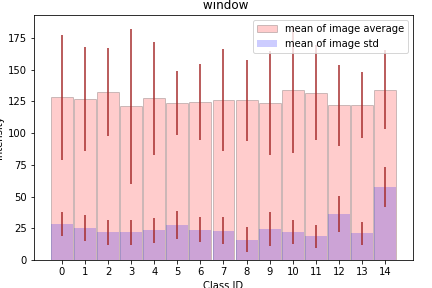
\includegraphics[width=0.80\linewidth]{Distribution_of_image_averages_and_standard_deviations_per_class}
    \caption{Distribution of image means and standard deviations per class window.}
	\label{fig:distImgAvgAndStd}
\end{figure}

\begin{figure}[h]
	\centering
    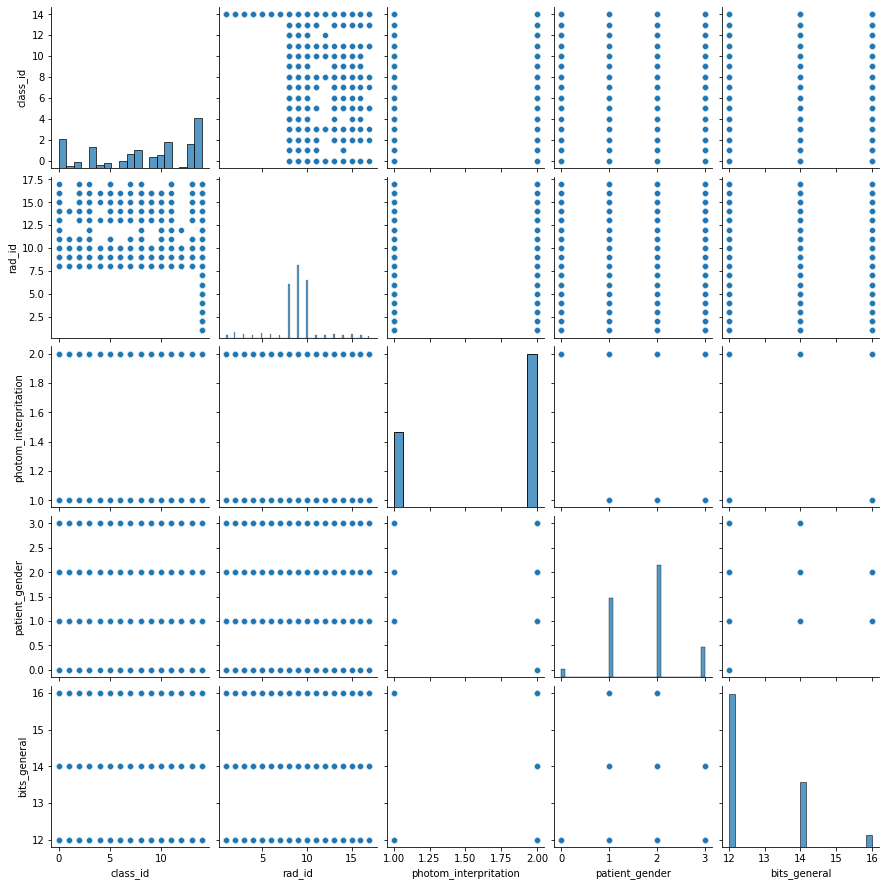
\includegraphics[width=0.80\linewidth]{pairplot}
    \caption{Pairwise plot of image metadata: image type, patient gender, image bit depth, radiologist findings, and radiologist ID.}
	\label{fig:pairplot}
\end{figure}

\begin{figure}[h]
	\centering
    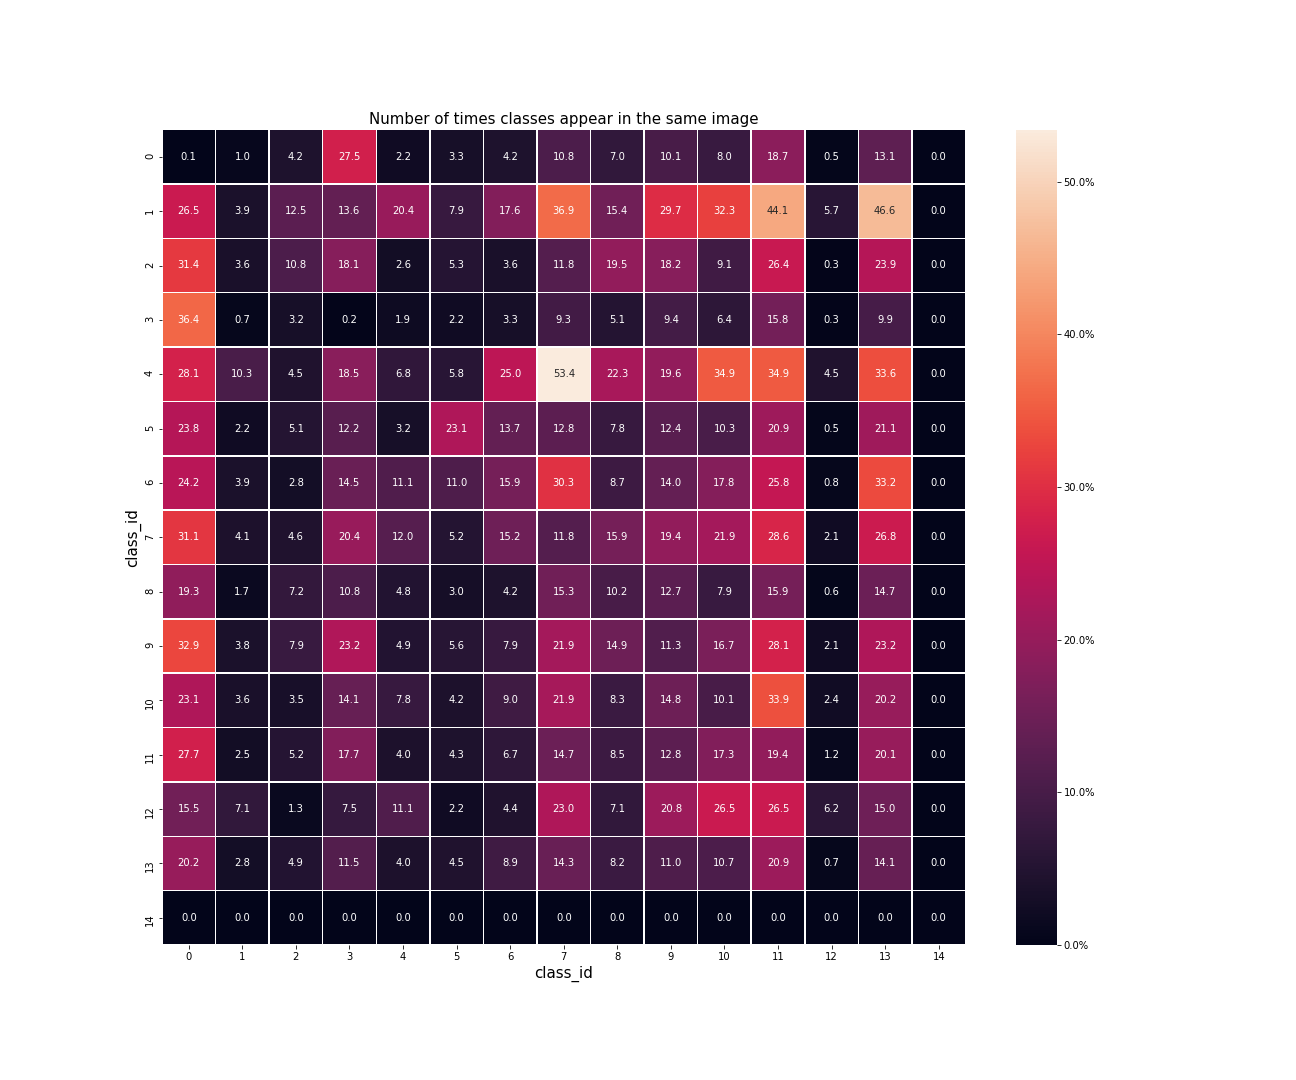
\includegraphics[width=0.80\linewidth]{NumClassAppearSameImg}
    \caption{Number of times classes appear in together in the same image.}
	\label{fig:NumTimesClassesAppearSameImg}
\end{figure}

In order to discover if some classes tend to appear at the same spot in image, the distribution of locations for each class was plotted. Firstly, the center of bounding box was calculated for each entry in the CSV file and then it was scaled to accommodate the differences in images’ sizes. Secondly, the locations of the center for each class were accumulated. And lastly, the distributions were plotted and their corresponding means and standard deviations were calculated. The distributions for each class are presented in Figure \ref{fig:distBB}.

As can be seen from the figure, classes Aortic enlargement and Cardiomegaly tend to appear roughly at the same spot. In addition, compared to other classes they have the lowest standard deviations. The reason for this is that according to the nature of diseases, the first finding has to be located in the upper part of Aorta while the second in the heart area. Further, classes Consolidation and ILD tend to appear in the bronchi part of an image.  In contrast, the possible positions of other findings are rather sparse: class Other Lesion is evenly distributed across the image and the rest of the classes are primarily distributed in the lung area. Thus, if a trained model has a lot of false positives for several mentioned classes, they can be easily filtered out by their location. 

We also decided to analyze the pixelation and brightness of images in the dataset. First of all, the distribution of average brightness of images was plotted. This was done by scaling the value of image pixels using the maximum value that can be stored in pixels, i.e. dividing image by two to the power of image bit depth. The mean pixel intensity was also calculated for each image. The distribution of average image brightness is presented in Figure \ref{fig:distImgBrightness}.

It can be concluded that the mean brightness of images is located around the intensity of 127. However, the standard deviation is rather high, meaning that some images in the dataset are very bright or very dark. Thus, it becomes necessary to center the intensity of all images around the same value. 

Next, the distribution of mean standard deviation of intensity inside the bounding boxes of each class was plotted. This was done in order to discover if some classes tend to appear in bright or dark regions of image, and how much the intensity varies on average for each class. In this way, the mean of pixels’ values was calculated for each class separately. The same was done with the standard deviation of intensity inside each window. Since the last class has the full image associated with it, the mentioned values were calculated for the entire images. The resulting distribution is presented in Figure \ref{fig:distImgAvgAndStd} Therefore, based on this distribution it can be concluded that image brightness inside the bounding boxes is roughly the same across the classes.  The same applies to image standard deviations.

As a next step of data analysis, some metadata taken from the images and data from the CSV file were grouped together. The correlation table was created together with pairwise graphs (Figure \ref{fig:pairplot}). This allows us to see if there are any correlations between the features. As can be seen in Figure \ref{fig:pairplot}, there are no meaningful correlations between the data, except a slight correlation between the radiologist and class IDs, and image type and depth.  Indeed, as seen from the pairwise plot, the radiologists who have IDs from 1 to 7 predict only No finding class, they have never predicted any other class. This also will be taken into account during the preprocessing step. The correlation between image type and depth can be explained by the fact that different imaging devices were used that had different presets.

Given that several different classes might appear in the same image, it is worth analysing which classes appear together. To achieve this, Figure \ref{fig:NumTimesClassesAppearSameImg} plots the number of times two classes appear together in image, divided by the total number of instances of a row class. For example, class 1 appears together with class 13 46\% of the time. It can be concluded that a majority of classes may show up together in an image. Also, as can be seen from the table, class 14 which corresponds to the No finding class, never appears together with other classes, meaning that radiologists are always certain that there are no findings. 

It was indicated in the Kaggle competition that the training dataset contains labels from multiple radiologists for each image. This means that for the same image, there are multiple “correct” targets. Fundamentally, we identified that this could be a source of confusion when training the network. Of course, the network can only make one prediction on an image - so unless all the radiologist labels are identical, there will be some amount of loss regardless of the network's prediction. The size of this loss would depend on how similar the labels from the radiologists were. For this reason, we deemed it necessary to investigate how the labels from multiple radiologists differed. The group created a python script which iterated through each unique image in the training set and compared the classes assigned to the image by radiologists. It was found that out of the 15,000 unique images in the training set, 3,718 had some disagreement of abnormalities assigned to the image. This script was however unable to account for the location of abnormalities- so if in one scan radiologist A identified a nodule at the top right of the image, but radiologist B identified a nodule at the bottom left, this would be considered to be the same class assignment by radiologists. For this reason we consider that 3,718 of 15,000 scans is somewhat of an underestimate of the disagreement among radiologists.

\subsection{Preprocessing}

\subsubsection{Label Preprocessing}
In order to address the problem of disagreements between radiologists, our label preprocessing was done in the following way. Assume that three doctors predicted the same class in an image. If the IoU (see Section V. metrics) score for any two bounding boxes was higher than 0.5, then it was assumed that the radiologists saw the same finding in the same spot. If two or more radiologists voted for the same class at the same spot, then their boxes were averaged and this averaged box was used to train our model. A demonstration of this procedure is given in Figure \ref{fig:radiologist_voting}. Figure \ref{fig:label_decrease} shows how the number of labels decreased by a factor of 4 after this process.

\subsubsection{Image Preprocessing and Augmentations}
For this step, we first converted all images from DICOM (Digital Imaging and Communication in Medicine) format to a multidimensional array. This was necessary since DICOM’s store pixel values on an exponential scale which is only resolved by standard DICOM viewers. To save space and time during training, all images were downscaled to a maximum of 1024 pixels along the longest axis. This way of downscaling kept the aspect ratio the same pre and post scaling for all images. All images were normalized to a mean of 0.4 and a standard deviation of 0.1. This process ensured that brightness distribution was relatively similar across all images. The values outside of [0,1] were clipped. Second, we applied image augmentation to all training images with the albumentations python package. Image augmentation is a popular technique to artificially increase the amount of data available to train a network \cite{perez2017effectiveness}. Specifically, our transformations include flipping images along the X-axis, rotating images between 0 and 20 degrees, and rescaling. We convert all relevant data including image arrays, bounding box data, radiologist findings, and radiologist IDs into PyTorch tensors to feed into our model. Since label preprocessing had severely diminished the number of viable observations for some classes, we used data augmentation to create new images. Three types of augmentations were used: random gamma, rotation in [-5, 5] range and random brightness/contrast. Figure \ref{fig:img_preprocessing_aug} illustrates all three of these augmentations applied to an image. 

\subsubsection{Class Distribution and Train/Validation Split}
Our goal was to create a train set where each class had at least 500 instances. As you can see in Figure \ref{fig:label_decrease}, some classes of abnormalities are severely underrepresented. We generated a sufficient number of images from those underrepresented classes using the augmentations described above, generating a new distribution of class labels presented in Figure \ref{fig:class_distribution}. Through this process, we used only 2,400 images out of the 15,000 images in the original dataset. By balancing the class distribution and preprocessing the class labels (filtering out disagreements), we were able to avoid using the vast majority of images which were either “no finding” or lacked radiologist consensus. 

\begin{figure}[h]
	\centering
    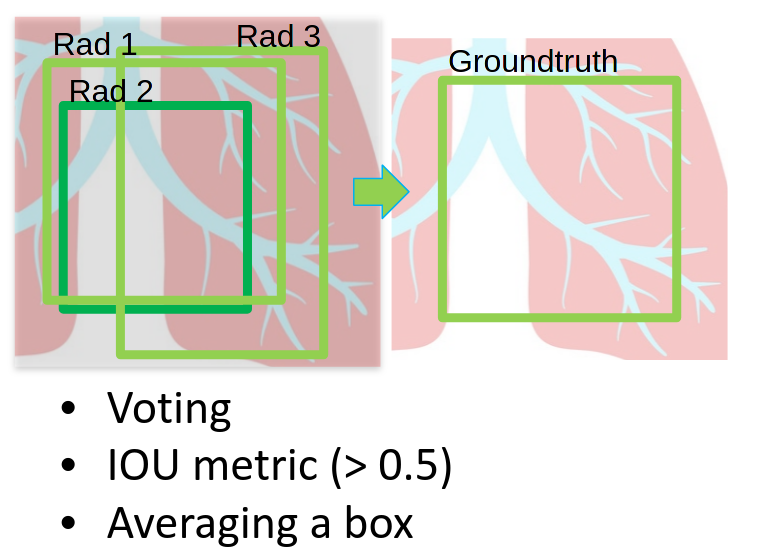
\includegraphics[width=0.80\linewidth]{radiologist_voting}
    \caption{Voting and averaging procedure for radiologist bounding boxes.}
	\label{fig:radiologist_voting}
\end{figure}

\begin{figure}[h]
	\centering
    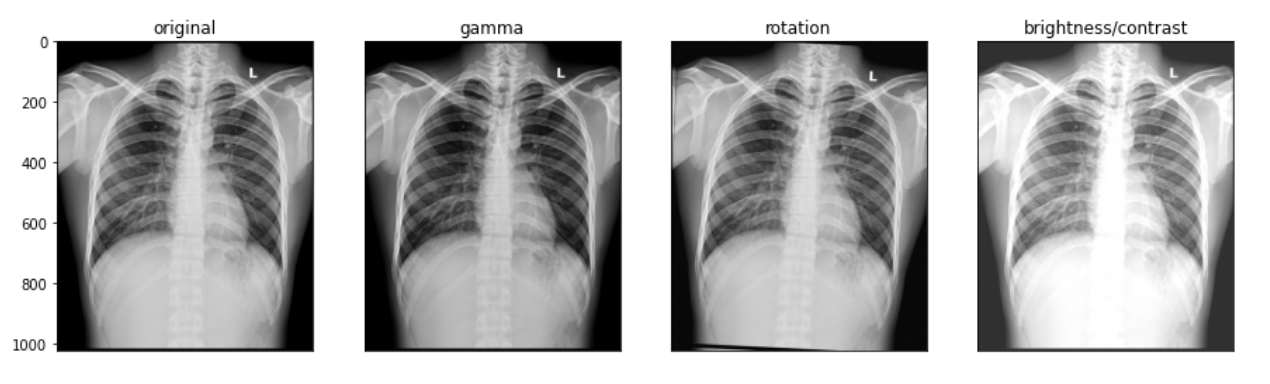
\includegraphics[width=0.80\linewidth]{img_preprocessing_aug}
    \caption{Image augmentation with original (left), gamma (middle-left), rotation (middle-right) and brightness/contrast (right) augmentations applied.}
	\label{fig:img_preprocessing_aug}
\end{figure}

\begin{figure}[h]
	\centering
    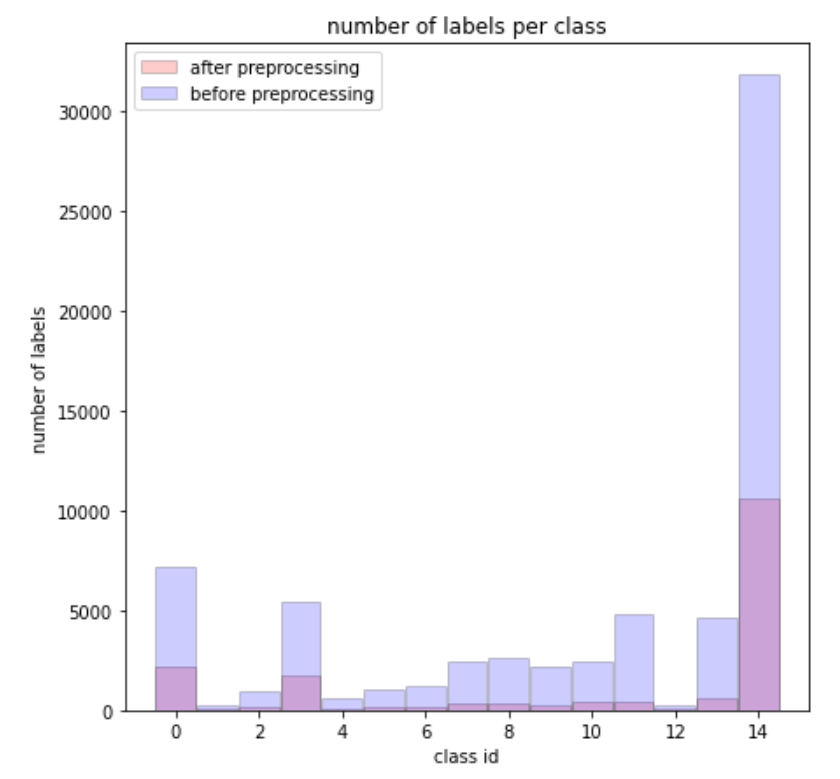
\includegraphics[width=0.80\linewidth]{label_decrease}
    \caption{Number of labels pre and post processing.}
	\label{fig:label_decrease}
\end{figure}

\begin{figure}[h]
	\centering
    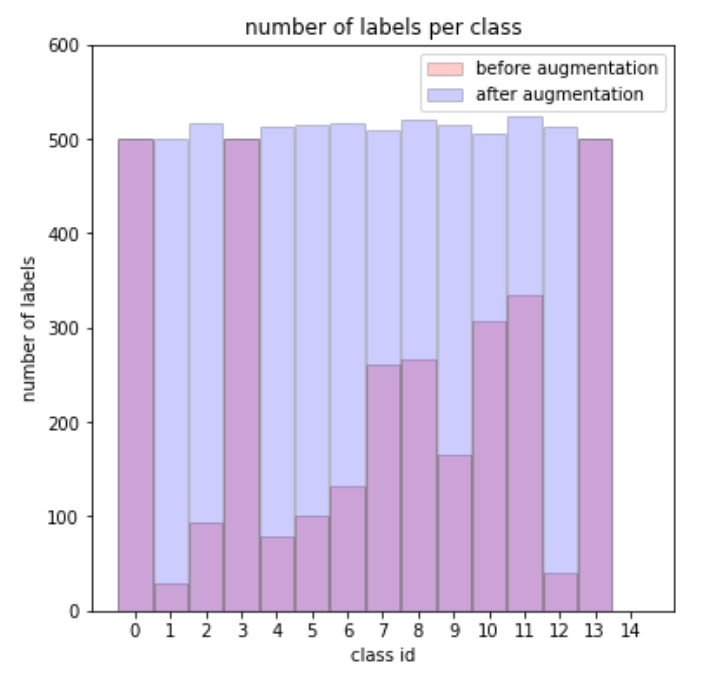
\includegraphics[width=0.80\linewidth]{class_distribution}
    \caption{Resulting class frequency distribution.}
	\label{fig:class_distribution}
\end{figure}

\subsection{Models}
As discussed in the related work, R-CNN and YOLO models are an ideal choice for object detection with localization tasks. In totoal, we trained four models. Three were variations of RCNN with differnent backbones: ResNet50-FPN, high resolution MobileNetV3Large and low resolution MobileNetV3Large, and the fourth was YOLO.

\subsection{Hyperparameter Tuning}
\subsubsection{R-CNN Models}
Our hyperparameter space includes boolean values for using pre-trained Faster R-CNN models and pre-trained backbone networks for each model. Pre-trained Faster R-CNN models mean reusing the weights of an entire Faster R-CNN network that was previously trained on the COCO train2017 dataset. This option applies to each of the three models discussed above. We also have the option of using pre-trained backbone networks for both convolutional networks (ResNet and MobileNetV3).  If true, weights were reused from each network previously trained on the Imagenet dataset. In addition to these hyperparameters, we will also tuned the number of trainable backbone layers when using a pre-trained backbone network is true. This parameter changes the number of non-frozen layers starting from the final block that are able to be re-trained using data specific to our task. We had the freedom of changing zero to all hidden layers to be non-frozen. In total four hyperparameters were tuned for each of the Faster R-CNN models tested. The hyperparameters together with their tested values are presented in Table \ref{tab:HyperparamVals}. Hyperparameters were tuned using gird search, and the best model was chosen based on the validation loss score. The best hyperparameters for each of the tested models together with their loss values are presented in Table \ref{tab:HyperparamResults}. 
\subsubsection{YOLO Model}
For YOLO, the hyperparameter tuning was done using the hyperparameter evolution algorithm. This is a stochastic population based method to find a global minimum of candidate spaces, and is able to efficiently search through a large number of candidate spaces. The results of the hyperparameter evolution is show in Figure \ref{fig:yolo_tuning}. For this tuning process, the best model was selected based on validation loss score. 

\begin{table}[]
\centering
\caption{\label{tab:HyperparamVals}Hyperparameters and values.}
\begin{tabular}{|l|l|}
\hline
Hyperparameter   & Values                    \\ \hline
Number of epochs & {[}1,2{]}                 \\ \hline
Learning rate    & {[}0.001, 0.005, 0.01{]}  \\ \hline
Momentum         & {[}0.9, 0.95{]}           \\ \hline
Starting weights & {[}Pre-trained, random{]} \\ \hline
\end{tabular}
\end{table}

\begin{table}[]
\centering
\caption{\label{tab:HyperparamResults}R-CNN Hyperparameter Tuning Results}
\resizebox{\columnwidth}{!}{\begin{tabular} {|l|l|l|l|l|l|}
\hline
\multicolumn{1}{|c|}{\multirow{Model}} & \multicolumn{4}{c|}{Hyperparameters} & \multirow{Loss Value} \\ \cline{2-5}
\multicolumn{1}{|c|}{} & \multicolumn{1}{c|}{Epoch} & \multicolumn{1}{c|}{Learning Rate} & \multicolumn{1}{c|}{Momentum} & \multicolumn{1}{c|}{Starting Weights} &  \\ \hline
ResNet50-FPN & 1 & 0.005 & 0.95 & Random & 0.153 \\ \hline
MobileNetV3Large320p & 1 & 0.01 & 0.9 & Pre-trained & 0.108 \\ \hline
MobileNetV3Large180p & 1 & 0.001 & 0.95 & Pre-trained & 0.181 \\ \hline
\end{tabular}}
\end{table}

\begin{figure}[h]
	\centering
    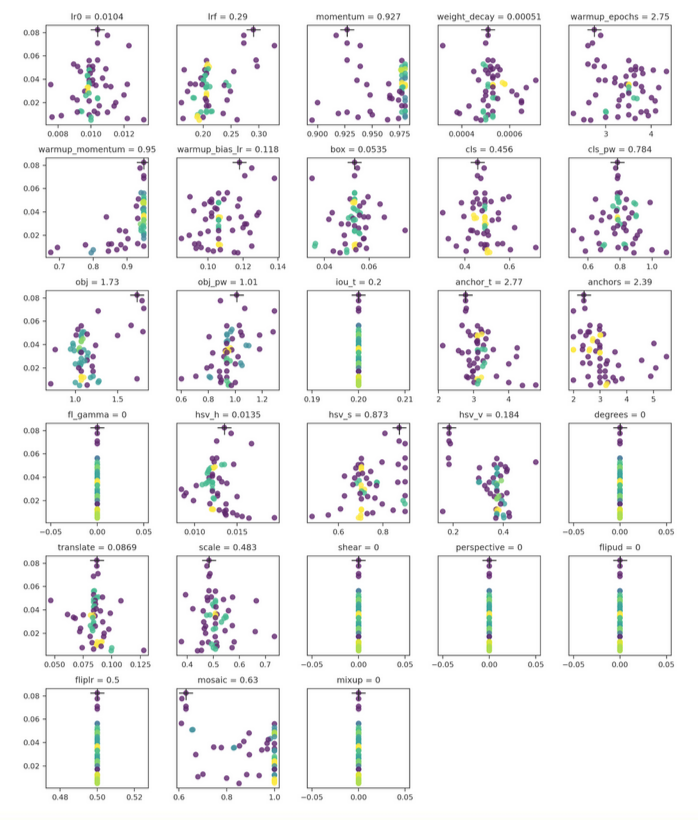
\includegraphics[width=0.80\linewidth]{yolo_tuning}
    \caption{YOLO Hyperparameter Tuning Results}
	\label{fig:yolo_tuning}
\end{figure}


\subsection{Training and Validation}
\subsubsection{R-CNN Models}
Based on the validation loss score from the hyperparamter search, the best model out of three RCNNs is MobileNetV3 Large. This model and its optimized hyperparameters was trained on the augmented training set. This model plateaud very quickly and the mAP score on the Kaggle test set is only 0.052. Its training and validation losses are presented in Figure \ref{fig:train_val_frcnn_optimal}.

\subsubsection{YOLO Models}
Figure \ref{fig:yolo_results} shows the YOLO metrics we computed through training. Not only did the model score a high mAP and low validation loss, it also convereged in just 35 epochs. We found that our YOLO model out-performed all three R-CNN models based on the validation loss score. We evaluated our best performing YOLO model from the hyperparameter search on the validation set and generated the confusion matrix shown in Figure \ref{fig:yolo_conf_matrix}.

\subsubsection{Model Selection}
Given that the YOLO model outcompeted all three R-CNN models according to validation loss, we prepared this model for submission. Sample predictions were plotted on unseen data in Figure \ref{fig:sample_predictions}. In this image, the ground truth labels are provided on the left with the predicitions from our YOLO model on the right. We can see that despite the complexity of the problem, the model is able to detect and localize findings moderately well. 

\begin{figure}[h]
	\centering
    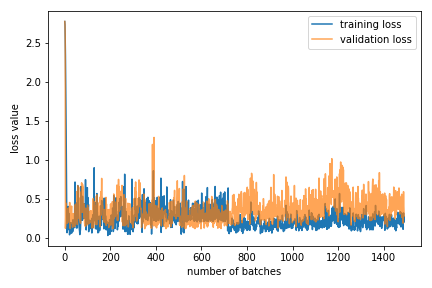
\includegraphics[width=0.80\linewidth]{TrainValLossFrcnnMobilenet_v3_large_320_fpn}
    \caption{Training and validation loss for the optimal hyperparameters of the Faster RCNN MobileNetV3 Large model.}
	\label{fig:train_val_frcnn_optimal}
\end{figure}

\begin{figure}[h]
	\centering
    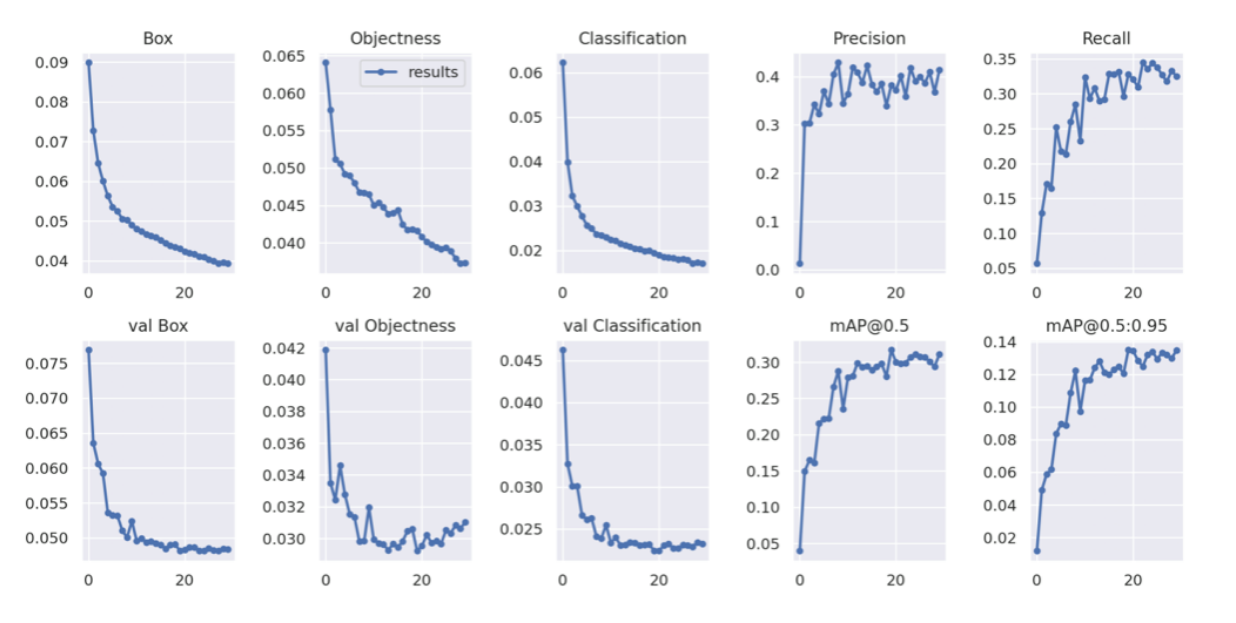
\includegraphics[width=0.80\linewidth]{yolo_results}
    \caption{YOLO training metrics computed.}
	\label{fig:yolo_results}
\end{figure}

\begin{figure}[h]
	\centering
    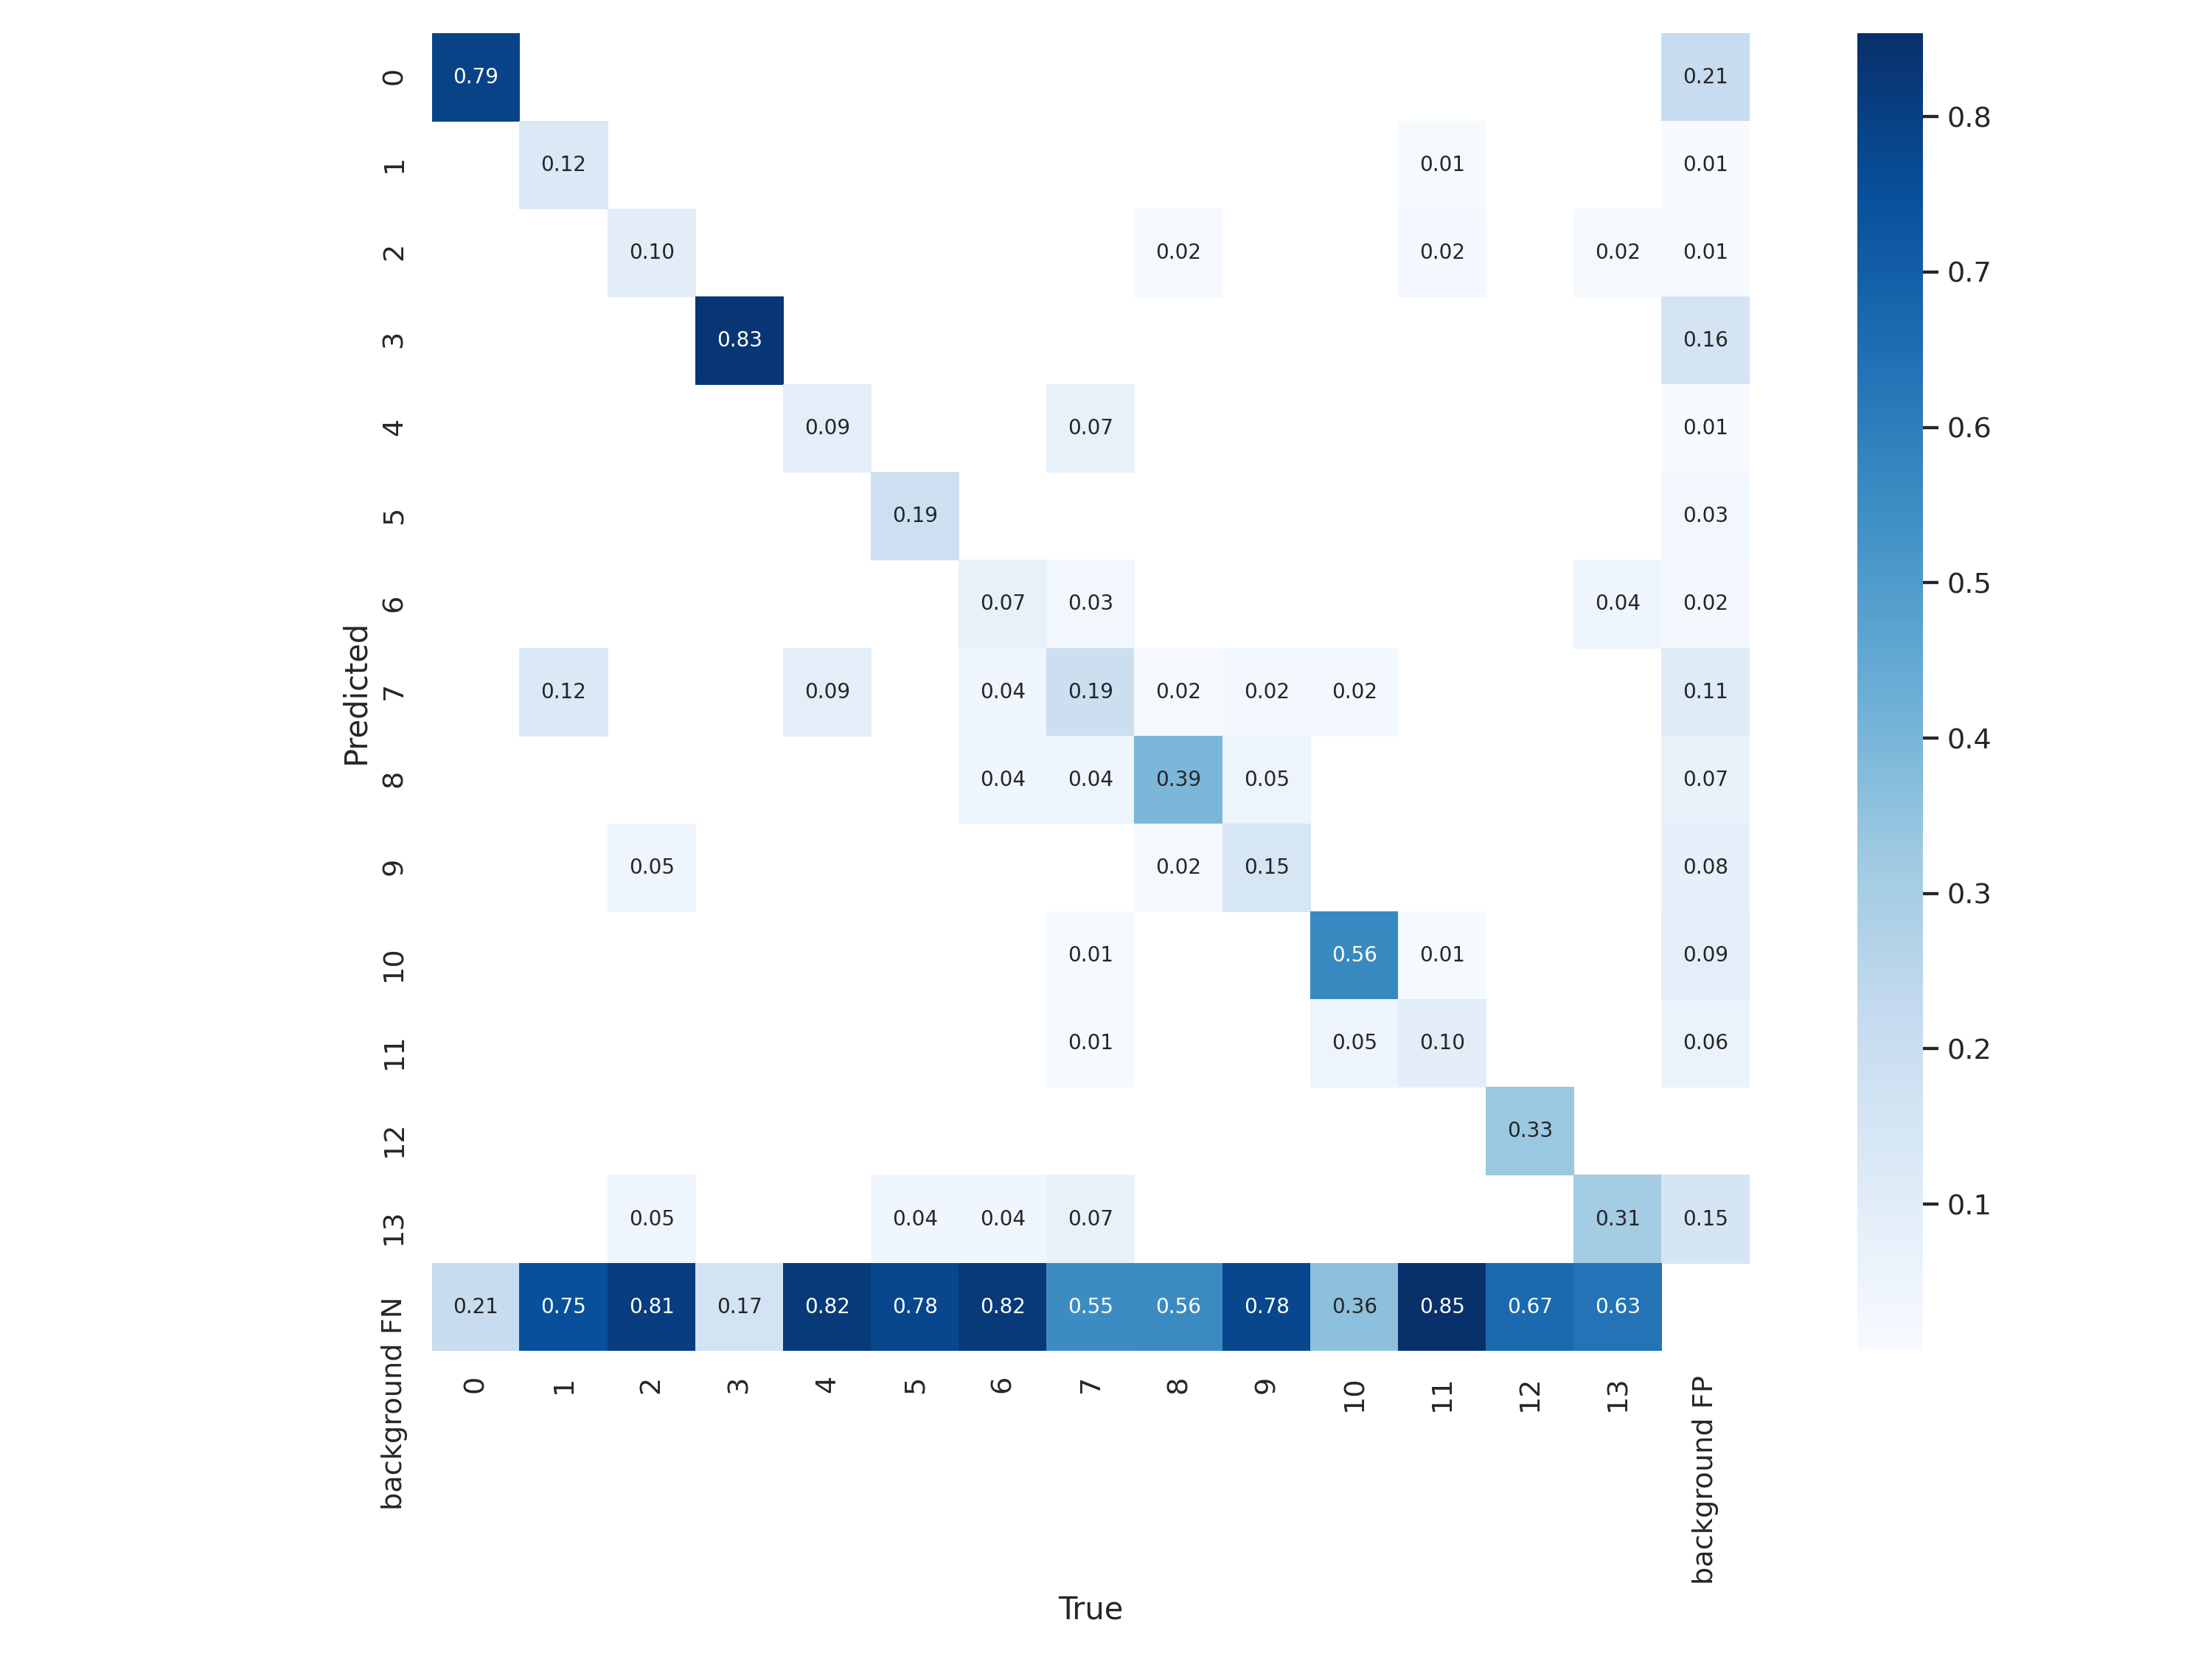
\includegraphics[width=0.80\linewidth]{yolo_conf_matrix}
    \caption{Confusion matrix representing the performance of best YOLO model on validation set.}
	\label{fig:yolo_conf_matrix}
\end{figure}

\begin{figure}[h]
	\centering
    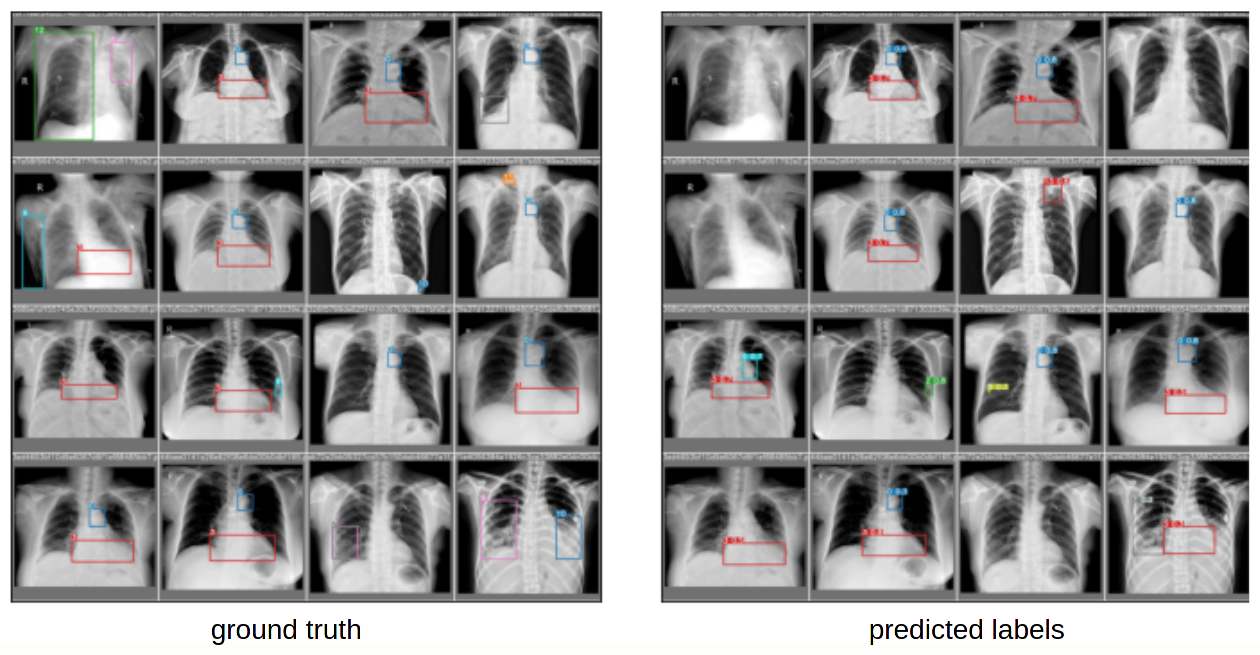
\includegraphics[width=0.80\linewidth]{sample_predictions}
    \caption{Sample predictions for YOLO on unseen images. Ground truth labels (left), predicted labels (right).}
	\label{fig:sample_predictions}
\end{figure}

\section{Results and Analysis} \label{results_and_analysis}
\subsection{Metrics}
From the literature we surveyed, the default and most popular metric used to measure the accuracy of Faster R-CNN object detectors is mean average precision (mAP). mAP computes the average intersection over union thresholds (IoU) for the set of predicted bounding boxes and ground truth boxes across images in a dataset. Formally, the IoU for ground truth box A and predicted box B is defined as follows: \[IoU(A,B) = \frac{A \cap B}{A \cup B} \]

In the literature, the most common threshold to satisfy intersection has been 0.5. In other words, a predicted object is considered correct if its intersection over union with a ground truth object is greater than or equal to 0.5. For each pair of boxes, a precision value is calculated as: \[ \frac{TP}{TP+FP+FN} \]

The average precision of a single image can thus be calculated as the mean of the precision values for each object in an image, and can be calculated as: \[ \frac{1}{n} \sum_{i=1}^{n}\frac{TP_i}{TP_i+FP_i+FN_i} \]

\subsection{Benchmarking & Expected Results}
We submitted our YOLO model as our final model in the competition. We ended up scoring a mAP of 24.6\% on the withheld test set, placing us in the top 26\% of all participants. The top team scored just 10 percentage points over us.

\section{Future Work} \label{future_work}
As reflected by the overall low competition scores, we found this problem to be difficult because of the lack of consensus in the training data between radiologists. We took extensive steps to resolve conflicting opinions, and we have a few more ideas of things we can try.
\begin{itemize}
    \item We could try combining and averaging the predictions from all four networks in an ensemble network style.
    \item We could use alternative voting schemes as a hyperparameter for the models, varying between minority sufficiency, majority sufficiency, or an all-or-nothing style where no disagreements can be present in order to admit a detected abnormality into the training process.
    \item We could try 2-class classification, where we first determine whether there is some finding or no finding at all, and only if there is some finding perfect detection and localization on that finding.
    \item We noticed that prediction confidences for some classes were very low, so we could do extensive post-processing on those features to try improve the models overall performance
    \item We can examine which radiologists in the train set had findings most consistent with the test set, so in other words were the most accurate when labelling independently, and train our models more heavily on them. 
\end{itemize}
Overall we are proud of the results we achieved but feel there are many opportunities to further improve.

\section{Appendix} \label{appendix}
\subsection{Contributions}
Technical contributions to the project were as follows: Kanstantsins contributions include the exploratory data analysis and the data preprocessing pipeline. He was also responsible for the implementation of YOLO and R-CNN models. Kyle was responsible for the description of the YOLO models along with a review of the previous contributions made to the model, and contributed to the exploratory data analysis and R-CNN model implementation. Christopher was responsible for the description of the R-CNN models used along with a review of the previous contributions made to those models, and also contributed to the data preprocessing efforts and the implementation of R-CNN. Equal contributions were made to all other sections of this report and project presentation.
\subsection{Bitbucket Repository}
Our Bitbucket repository with the code for our final project can be found here: https://bitbucket.org/christam88/group19-final-project/src/main/ 

\bibliographystyle{IEEEtran}
%\IEEEtriggeratref{24}
\bibliography{references}

\end{document}
